\documentclass[11pt,a4paper]{article}

% ------------------------------------------------------------------
% Packages
% ------------------------------------------------------------------
\usepackage[utf8]{inputenc}
\usepackage[T1]{fontenc}
\usepackage{lmodern}
\usepackage[margin=2.5cm]{geometry}
\usepackage{amsmath,amssymb,amsthm,mathtools}
\usepackage{booktabs}
\usepackage{graphicx}
\usepackage{xcolor}
\usepackage{listings}
\usepackage{algorithm}
\usepackage{algpseudocode}
\usepackage{caption}
\usepackage{subcaption}
\usepackage{pgfplots}
\usepgfplotslibrary{groupplots}
\pgfplotsset{compat=1.17}
\usepackage[colorlinks=true,linkcolor=blue!60!black,citecolor=blue!60!black,urlcolor=blue!60!black]{hyperref}
\usepackage{cleveref}

% ------------------------------------------------------------------
% Theorems
% ------------------------------------------------------------------
\newtheorem{proposition}{Proposition}[section]
\theoremstyle{remark}
\newtheorem{remark}{Remark}[section]

% ------------------------------------------------------------------
% Macros
% ------------------------------------------------------------------
\newcommand{\E}{\mathbb{E}}
\newcommand{\Q}{\mathbb{Q}}
\newcommand{\ind}{\mathbf{1}}
\newcommand{\dd}{\mathrm{d}}
\newcommand{\code}[1]{\texttt{#1}}
\newcommand{\todo}[1]{\textcolor{red}{\textbf{[TODO: #1]}}}

% Figures exported from Produits/Digitale/digital_pricer.ipynb into figures/.
% A framed placeholder is printed while a file is missing, so that the document always compiles.
\newcommand{\figfile}[2]{%
  \IfFileExists{figures/#1}{\includegraphics[width=#2]{figures/#1}}%
  {\fbox{\parbox[c][4cm][c]{#2}{\centering\small missing figure:\\ \texttt{figures/#1}}}}}

\lstset{basicstyle=\ttfamily\footnotesize, keywordstyle=\color{blue!70!black}, commentstyle=\color{gray},
        stringstyle=\color{teal}, frame=single, breaklines=true, language=Python, showstringspaces=false}

% ------------------------------------------------------------------
\title{Digital Options: Pricing, Greeks and Hedging}
\author{Elias Benguedda}
\date{October 2026}

\begin{document}
\emergencystretch=3em
\maketitle

\begin{abstract}
This paper studies the pricing of digital options under several models
(Black--Scholes, Heston and local-stochastic volatility) for the European,
Bermudan and American exercise styles. We then analyse the associated Greeks
and the hedging and replication of these options, and conclude with a
risk-management assessment.
\end{abstract}

\clearpage
\tableofcontents
\newpage

% ==================================================================
\section{Introduction}
\label{sec:intro}
% ==================================================================

\subsection{Motivation}

Digital options are liquid instruments, especially on FX markets, but they are
not vanilla products: their discontinuous payoff makes both their pricing and
their hedging delicate, and dedicated pricers are required.

\subsection{Outline}

Section~\ref{sec:products} describes the products and their model-free
properties. Section~\ref{sec:bs} derives their prices under the Black--Scholes
model, which serves as a benchmark. Section~\ref{sec:data} presents the market
data and the calibrated model used in the rest of the paper.
Section~\ref{sec:heston} prices digital options under the Heston model,
Section~\ref{sec:greeks} studies their Greeks and Section~\ref{sec:hedging}
their hedging.

% ==================================================================
\section{Digital Options}
\label{sec:products}
% ==================================================================

Digital options, also called binary options, pay a fixed coupon when a trigger
event occurs. There are two kinds of digital options: cash-or-nothing (CON) and
asset-or-nothing (AON) options. Many underlyings are possible, such as a single
stock, an index or a basket. To keep the descriptions simple, we present the
call versions; the put versions are treated in the associated notebook. In the
following, $K$ denotes the trigger level (or strike) and $Q$ the cash amount.

\subsection{Cash-or-Nothing Options}

The European CON call is the simplest digital option. It pays the cash amount
$Q$ at maturity if the underlying finishes above the strike
(Figure~\ref{fig:payoff-con}):
\begin{equation}
  \mathrm{CON}_T = Q\,\ind_{\{S_T \geq K\}}.
  \label{eq:con-payoff}
\end{equation}

\begin{figure}[htbp]
\centering
\begin{tikzpicture}
\begin{axis}[
    axis lines=middle,
    xlabel={$S_T$}, ylabel={Payoff},
    xmin=0, xmax=10, ymin=0, ymax=6,
    xtick={4}, xticklabels={$K$},
    ytick={3}, yticklabels={$Q$},
    width=9cm, height=7cm,
    every axis x label/.style={at={(ticklabel* cs:1)}, anchor=west},
    every axis y label/.style={at={(ticklabel* cs:1)}, anchor=south},
]
    % Zero payoff below K
    \addplot[very thick, blue, domain=0:4] {0};
    % Payoff Q above K
    \addplot[very thick, blue, domain=4:9.5] {3};
    % Jump at K
    \draw[dashed, gray] (axis cs:4,0) -- (axis cs:4,3);
    \fill[blue] (axis cs:4,3) circle (2.5pt);
    \draw[blue, fill=white] (axis cs:4,0) circle (2.5pt);
\end{axis}
\end{tikzpicture}
\caption{Payoff of a European cash-or-nothing call.}
\label{fig:payoff-con}
\end{figure}

\subsection{Asset-or-Nothing Options}

The European AON call pays the value of the underlying at maturity if this
value is above the strike (Figure~\ref{fig:payoff-aon}):
\begin{equation}
  \mathrm{AON}_T = S_T\,\ind_{\{S_T \geq K\}}.
  \label{eq:aon-payoff}
\end{equation}

\begin{figure}[htbp]
\centering
\begin{tikzpicture}
\begin{axis}[
    axis lines=middle,
    xlabel={$S_T$}, ylabel={Payoff},
    xmin=0, xmax=10, ymin=0, ymax=10,
    xtick={4}, xticklabels={$K$},
    ytick={4}, yticklabels={$K$},
    width=9cm, height=7cm,
    every axis x label/.style={at={(ticklabel* cs:1)}, anchor=west},
    every axis y label/.style={at={(ticklabel* cs:1)}, anchor=south},
]
    % Zero payoff below K
    \addplot[very thick, blue, domain=0:4] {0};
    % Payoff S_T above K
    \addplot[very thick, blue, domain=4:9.5] {x};
    % Jump at K
    \draw[dashed, gray] (axis cs:4,0) -- (axis cs:4,4);
    \fill[blue] (axis cs:4,4) circle (2.5pt);
    \draw[blue, fill=white] (axis cs:4,0) circle (2.5pt);
\end{axis}
\end{tikzpicture}
\caption{Payoff of a European asset-or-nothing call.}
\label{fig:payoff-aon}
\end{figure}

\subsection{Exercise Styles and Touch Options}

Both CON and AON options also exist in American and Bermudan versions, in which
the trigger is monitored not only at maturity but continuously, or on a
discrete set of dates, before maturity. Contracts typically specify a
monitoring of the trigger at each daily close. The coupon may then be paid
either when the trigger is hit or at maturity. As always for early-exercise
products, such options are harder to price because the exercise time is
unknown.

Path-dependent digitals come in several types:
\begin{enumerate}
  \item \textbf{One-touch:} pays if and only if the barrier is touched, either
        immediately or at maturity;
  \item \textbf{No-touch:} pays if and only if the barrier is never touched;
  \item \textbf{Double one-touch:} two barriers, pays if and only if either
        barrier is touched;
  \item \textbf{Double no-touch:} two barriers, pays if and only if neither
        barrier is touched.
\end{enumerate}
Their prices under the Black--Scholes model are derived in
Sections~\ref{subsec:bs-american} and~\ref{subsec:bs-bermudan}.

\subsection{Static Decomposition of the Vanilla Call}

The payoff of a vanilla call decomposes into digital payoffs:
\begin{equation}
  (S_T - K)^+ = S_T\,\ind_{\{S_T \geq K\}} - K\,\ind_{\{S_T \geq K\}}.
\end{equation}
By absence of arbitrage, a vanilla call is therefore worth an asset-or-nothing
call minus $K$ cash-or-nothing calls with $Q=1$, in any model. This relation is
made explicit under Black--Scholes in~\eqref{eq:vanilla-decomposition}.

\subsection{Replication by Call Spreads}
\label{subsec:call-spread}

A digital option can be seen as the limit of a call spread~\cite{Bouzoubaa2010}.
Consider a call spread with strikes $K-\epsilon$ and $K+\epsilon$, and a
digital call struck at $K$ paying $Q=1$. Then
\begin{equation}
  \text{Digital}(K)
  = \lim_{\epsilon \to 0} \frac{1}{2\epsilon}
    \bigl( \text{Call}(K-\epsilon) - \text{Call}(K+\epsilon) \bigr)
  = -\frac{\partial\, \text{Call}(K)}{\partial K}.
  \label{eq:call-spread-limit}
\end{equation}
Figure~\ref{fig:digital-callspread} illustrates the convergence of the call
spread payoffs to the digital payoff.

\begin{figure}[htbp]
\centering
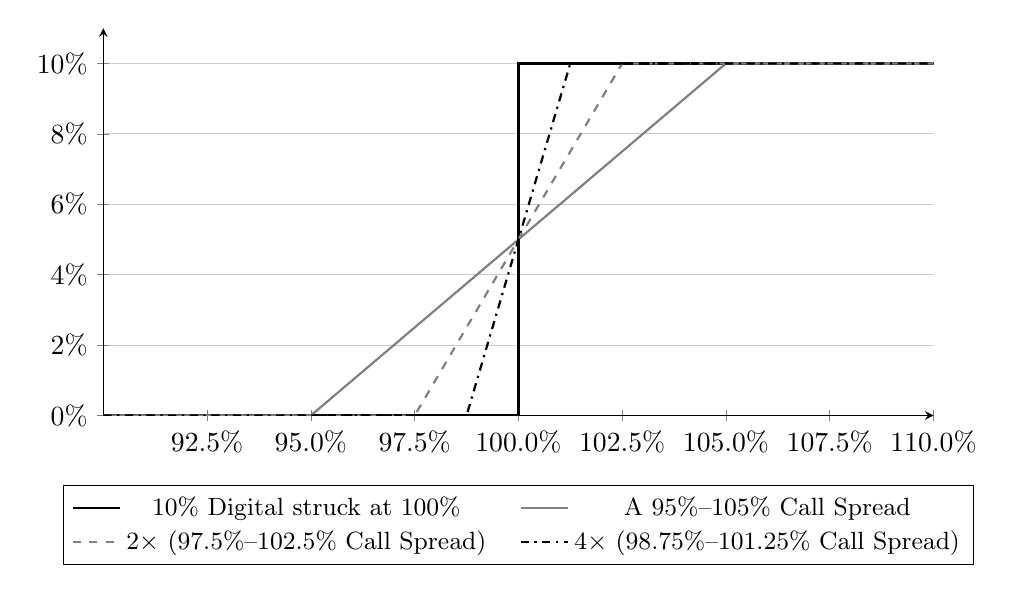
\begin{tikzpicture}
\begin{axis}[
    width=\textwidth, height=6.5cm,
    xmin=90, xmax=110, ymin=0, ymax=11,
    xtick={92.5,95,97.5,100,102.5,105,107.5,110},
    ytick={0,2,4,6,8,10},
    xticklabel={\pgfmathprintnumber[fixed,fixed zerofill,precision=1]{\tick}\%},
    yticklabel={\pgfmathprintnumber{\tick}\%},
    ymajorgrids=true,
    grid style={gray!40},
    axis x line=bottom, axis y line=left,
    legend style={
        at={(0.5,-0.18)}, anchor=north,
        legend columns=2, font=\small,
        /tikz/every even column/.append style={column sep=1em}
    },
]
    % 10% digital struck at 100%
    \addplot[black, thick] coordinates {(90,0) (100,0) (100,10) (110,10)};
    \addlegendentry{10\% Digital struck at 100\%}

    % 95%--105% call spread
    \addplot[gray, thick] coordinates {(90,0) (95,0) (105,10) (110,10)};
    \addlegendentry{A 95\%--105\% Call Spread}

    % 2 x 97.5%--102.5% call spread
    \addplot[gray, thick, dashed] coordinates {(90,0) (97.5,0) (102.5,10) (110,10)};
    \addlegendentry{$2\times$ (97.5\%--102.5\% Call Spread)}

    % 4 x 98.75%--101.25% call spread
    \addplot[black, thick, dash dot] coordinates {(90,0) (98.75,0) (101.25,10) (110,10)};
    \addlegendentry{$4\times$ (98.75\%--101.25\% Call Spread)}
\end{axis}
\end{tikzpicture}
\caption{A 10\% digital and three call spreads with different strikes. The closer the
call spread strikes are to the digital strike, the closer the payoff.}
\label{fig:digital-callspread}
\end{figure}

% ==================================================================
\section{Pricing under the Black--Scholes Model}
\label{sec:bs}
% ==================================================================

This section derives the prices of digital options in the Black--Scholes
framework~\cite{BlackScholes1973,Merton1973} for the three exercise styles
studied in this paper: European, American and Bermudan. Closed-form or
semi-closed-form expressions are available in each case, which makes the model
a natural benchmark for the stochastic volatility results of
Section~\ref{sec:heston}. The section ends with a discussion of why these
formulas are not sufficient for equity-index digitals.

% Figures use a logistic approximation of N(x) (max error ~1e-4),
% since pgfmath has no built-in normal CDF.

% ---------------------------------------------------------------------
\subsection{Model and Notation}
\label{subsec:bs-model}

Let $S_t$ denote the level of the underlying index. Under the risk-neutral
measure $\mathbb{Q}$, the index follows
\begin{equation}
  \mathrm{d}S_t = (r-q)\,S_t\,\mathrm{d}t + \sigma\,S_t\,\mathrm{d}W_t,
  \label{eq:bs-sde}
\end{equation}
where $r$ is the constant risk-free rate, $q$ the continuous dividend yield,
$\sigma$ the constant volatility and $W$ a standard Brownian motion. We write
$\tau = T-t$ for the time to maturity, $\nu = r - q - \tfrac{1}{2}\sigma^2$ for
the drift of $\ln S_t$, and
\begin{equation}
  d_1 = \frac{\ln(S_t/K) + \left(r - q + \tfrac{1}{2}\sigma^2\right)\tau}{\sigma\sqrt{\tau}},
  \qquad
  d_2 = d_1 - \sigma\sqrt{\tau}.
  \label{eq:d1d2}
\end{equation}
$N(\cdot)$ and $n(\cdot)$ denote the standard normal cumulative distribution
and density functions. Two probabilities appear throughout this section:
\begin{equation}
  \mathbb{Q}\left(S_T \geq K \mid \mathcal{F}_t\right) = N(d_2),
  \qquad
  \mathbb{Q}^S\left(S_T \geq K \mid \mathcal{F}_t\right) = N(d_1),
  \label{eq:probas}
\end{equation}
where $\mathbb{Q}^S$ is the share measure, defined by
\begin{equation}
  \left.\frac{\mathrm{d}\mathbb{Q}^S}{\mathrm{d}\mathbb{Q}}\right|_{\mathcal{F}_T}
  = \frac{S_T\, e^{-(r-q)T}}{S_0}.
\end{equation}

% ---------------------------------------------------------------------
\subsection{European Digital Options}
\label{subsec:bs-european}

\subsubsection{Cash-or-Nothing Options}

A cash-or-nothing call (resp.\ put) with strike $K$ and cash amount $Q$ pays
$Q\,\mathbf{1}_{\{S_T \geq K\}}$ (resp.\ $Q\,\mathbf{1}_{\{S_T < K\}}$) at
maturity. Its price is the discounted risk-neutral probability of finishing in
the money:
\begin{align}
  D^{c}(S_t,K,\tau) &= e^{-r\tau}\,\mathbb{E}^{\mathbb{Q}}\!\left[Q\,\mathbf{1}_{\{S_T \geq K\}} \mid \mathcal{F}_t\right]
                     = Q\,e^{-r\tau}\,N(d_2), \label{eq:cash-call}\\
  D^{p}(S_t,K,\tau) &= Q\,e^{-r\tau}\,N(-d_2). \label{eq:cash-put}
\end{align}

\subsubsection{Asset-or-Nothing Options}

An asset-or-nothing call (resp.\ put) pays $S_T\,\mathbf{1}_{\{S_T \geq K\}}$
(resp.\ $S_T\,\mathbf{1}_{\{S_T < K\}}$). Changing numeraire to the share
measure gives
\begin{align}
  A^{c}(S_t,K,\tau) &= e^{-r\tau}\,\mathbb{E}^{\mathbb{Q}}\!\left[S_T\,\mathbf{1}_{\{S_T \geq K\}} \mid \mathcal{F}_t\right]
                     = S_t\,e^{-q\tau}\,N(d_1), \label{eq:asset-call}\\
  A^{p}(S_t,K,\tau) &= S_t\,e^{-q\tau}\,N(-d_1). \label{eq:asset-put}
\end{align}

\subsubsection{Parity Relations and Static Decomposition}

Since the call and put payoffs sum to a constant, the following parity
relations hold in any arbitrage-free model:
\begin{equation}
  D^{c} + D^{p} = Q\,e^{-r\tau},
  \qquad
  A^{c} + A^{p} = S_t\,e^{-q\tau}.
  \label{eq:digital-parity}
\end{equation}
Moreover, the payoff of a vanilla call decomposes as
$(S_T-K)^+ = S_T\,\mathbf{1}_{\{S_T \geq K\}} - K\,\mathbf{1}_{\{S_T \geq K\}}$,
so that, with $Q=1$,
\begin{equation}
  C(S_t,K,\tau) = A^{c}(S_t,K,\tau) - K\,D^{c}(S_t,K,\tau)
               = S_t\,e^{-q\tau}N(d_1) - K\,e^{-r\tau}N(d_2),
  \label{eq:vanilla-decomposition}
\end{equation}
which recovers the Black--Scholes formula. Digital options are therefore the
elementary building blocks of vanilla options.

\subsubsection{Replication by Call Spreads and the Role of the Smile}
\label{subsubsec:call-spread}

By~\eqref{eq:call-spread-limit}, a digital call with $Q=1$ is minus the
derivative of the call price with respect to the strike. With a flat
volatility, differentiating the Black--Scholes formula gives
$-\partial C/\partial K = e^{-r\tau}N(d_2)$, consistent
with~\eqref{eq:cash-call}. When the market quotes a strike-dependent implied
volatility $\sigma(K)$, the call price is
$C^{\mathrm{mkt}}(K) = C^{\mathrm{BS}}\bigl(K,\sigma(K)\bigr)$ and the chain rule
yields
\begin{equation}
  D^{c,\mathrm{mkt}}(K)
  = e^{-r\tau}N(d_2) - \mathcal{V}^{\mathrm{BS}}(K)\,\frac{\partial \sigma}{\partial K},
  \qquad
  \mathcal{V}^{\mathrm{BS}}(K) = S_t\,e^{-q\tau}\,n(d_1)\sqrt{\tau},
  \label{eq:smile-correction}
\end{equation}
where $d_2$ is evaluated at $\sigma(K)$ and $\mathcal{V}^{\mathrm{BS}}$ is the
vega of the vanilla call. Equity indices exhibit a negative skew
($\partial\sigma/\partial K < 0$), so the market price of a digital call is
\emph{higher} than its Black--Scholes price computed with $\sigma(K)$, and the
market price of a digital put is correspondingly lower. Pricing a digital with
a single volatility therefore ignores a first-order effect of the smile.

\subsubsection{Greeks}
\label{subsubsec:bs-greeks}

For a cash-or-nothing call with $Q=1$, differentiating~\eqref{eq:cash-call}
gives
\begin{align}
  \Delta^{c} &= \frac{\partial D^{c}}{\partial S}
              = \frac{e^{-r\tau}\,n(d_2)}{S\,\sigma\sqrt{\tau}}, \label{eq:digital-delta}\\
  \Gamma^{c} &= \frac{\partial^2 D^{c}}{\partial S^2}
              = -\frac{e^{-r\tau}\,n(d_2)\,d_1}{S^2\,\sigma^2\,\tau}, \label{eq:digital-gamma}\\
  \mathcal{V}^{c} &= \frac{\partial D^{c}}{\partial \sigma}
              = -\frac{e^{-r\tau}\,n(d_2)\,d_1}{\sigma}. \label{eq:digital-vega}
\end{align}
As for vanilla options, vega and gamma are linked by
$\mathcal{V}^{c} = \sigma\,S^2\,\tau\,\Gamma^{c}$. By the parity
relation~\eqref{eq:digital-parity}, the Greeks of the cash-or-nothing put are
the opposite of those of the call.

Three features distinguish these Greeks from those of a vanilla option
(Figures~\ref{fig:bs-digital-price} to~\ref{fig:bs-digital-vega}):
\begin{itemize}
  \item the delta is bell-shaped around the strike and, as $\tau \to 0$,
        converges to a Dirac mass at $K$: close to maturity, the hedge ratio
        becomes unbounded for an at-the-money digital;
  \item gamma and vega change sign at $d_1 = 0$, i.e.\ at
        $S = K e^{-(r-q+\sigma^2/2)\tau}$: they are positive when the option
        is out of the money and negative when it is in the money;
  \item consequently, a digital option is not a monotone bet on volatility:
        an increase in volatility raises the price of an out-of-the-money
        digital and lowers the price of an in-the-money one.
\end{itemize}
A systematic comparison with the Greeks obtained under stochastic volatility
is carried out in Section~\ref{sec:greeks}.

% --- Figure: price -----------------------------------------------------
\begin{figure}[htbp]
\centering
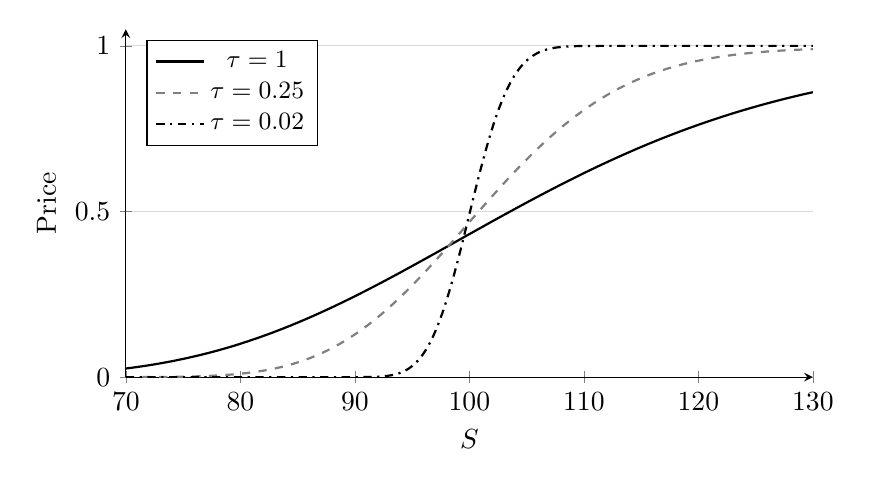
\begin{tikzpicture}
\begin{axis}[
    width=0.85\textwidth, height=6cm,
    xmin=70, xmax=130, ymin=0, ymax=1.05,
    xlabel={$S$}, ylabel={Price},
    ymajorgrids=true, grid style={gray!30},
    axis x line=bottom, axis y line=left,
    legend pos=north west, legend style={font=\small},
    samples=200,
    % Parameters: K = 100, r = 2%, q = 3%, sigma = 20%
    declare function={
      Ncdf(\x) = 1/(1+exp(-0.07056*\x*\x*\x - 1.5976*\x));
      dtwo(\s,\t) = (ln(\s/100) - 0.03*\t)/(0.2*sqrt(\t));
    },
]
  \addplot[black, thick, domain=70:130] {exp(-0.02*1)*Ncdf(dtwo(x,1))};
  \addlegendentry{$\tau = 1$}
  \addplot[gray, thick, dashed, domain=70:130] {exp(-0.02*0.25)*Ncdf(dtwo(x,0.25))};
  \addlegendentry{$\tau = 0.25$}
  \addplot[black, thick, dash dot, domain=70:130] {exp(-0.02*0.02)*Ncdf(dtwo(x,0.02))};
  \addlegendentry{$\tau = 0.02$}
\end{axis}
\end{tikzpicture}
\caption{Black--Scholes price of a cash-or-nothing call ($Q=1$) as a function
of the spot, for several maturities ($K=100$, $r=2\%$, $q=3\%$,
$\sigma=20\%$).}
\label{fig:bs-digital-price}
\end{figure}

% --- Figure: delta -----------------------------------------------------
\begin{figure}[htbp]
\centering
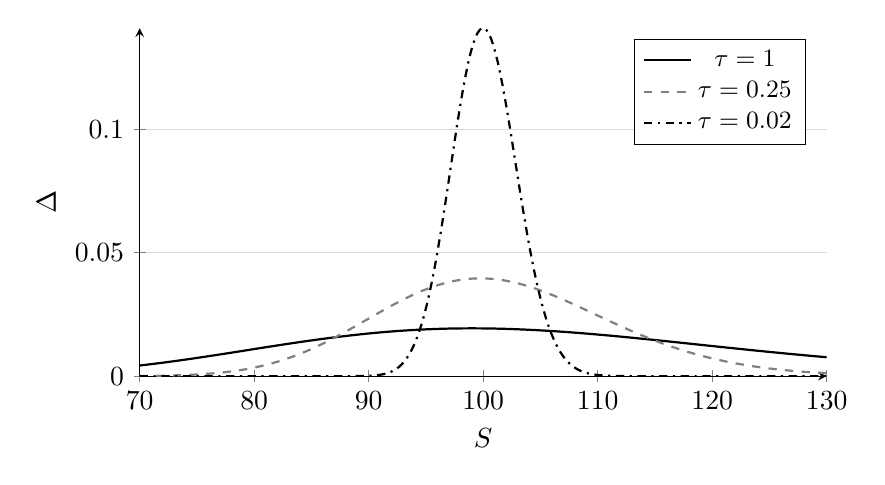
\begin{tikzpicture}
\begin{axis}[
    width=0.85\textwidth, height=6cm,
    xmin=70, xmax=130, ymin=0,
    xlabel={$S$}, ylabel={$\Delta$},
    ymajorgrids=true, grid style={gray!30},
    axis x line=bottom, axis y line=left,
    legend pos=north east, legend style={font=\small},
    scaled y ticks=false,
    yticklabel style={/pgf/number format/fixed, /pgf/number format/precision=2},
    samples=300,
    % Parameters: K = 100, r = 2%, q = 3%, sigma = 20%
    declare function={
      dtwo(\s,\t) = (ln(\s/100) - 0.03*\t)/(0.2*sqrt(\t));
      delta(\s,\t) = exp(-0.02*\t)*exp(-0.5*dtwo(\s,\t)*dtwo(\s,\t))
                     /(sqrt(2*pi)*\s*0.2*sqrt(\t));
    },
]
  \addplot[black, thick, domain=70:130] {delta(x,1)};
  \addlegendentry{$\tau = 1$}
  \addplot[gray, thick, dashed, domain=70:130] {delta(x,0.25)};
  \addlegendentry{$\tau = 0.25$}
  \addplot[black, thick, dash dot, domain=70:130] {delta(x,0.02)};
  \addlegendentry{$\tau = 0.02$}
\end{axis}
\end{tikzpicture}
\caption{Black--Scholes delta of a cash-or-nothing call ($Q=1$). The delta
concentrates around the strike as maturity approaches.}
\label{fig:bs-digital-delta}
\end{figure}

% --- Figure: gamma -----------------------------------------------------
\begin{figure}[htbp]
\centering
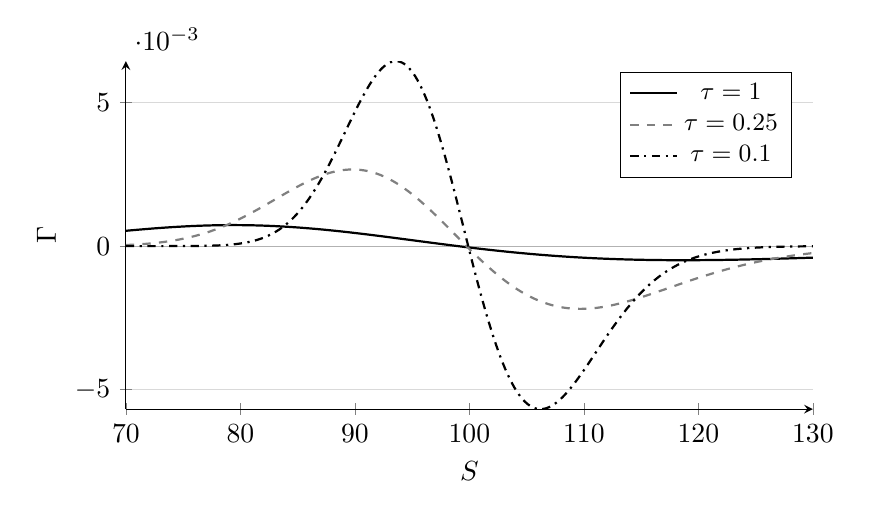
\begin{tikzpicture}
\begin{axis}[
    width=0.85\textwidth, height=6cm,
    xmin=70, xmax=130,
    xlabel={$S$}, ylabel={$\Gamma$},
    ymajorgrids=true, grid style={gray!30},
    axis x line=bottom, axis y line=left,
    legend pos=north east, legend style={font=\small},
    samples=300,
    % Parameters: K = 100, r = 2%, q = 3%, sigma = 20%
    declare function={
      dtwo(\s,\t) = (ln(\s/100) - 0.03*\t)/(0.2*sqrt(\t));
      done(\s,\t) = dtwo(\s,\t) + 0.2*sqrt(\t);
      gam(\s,\t)  = -exp(-0.02*\t)*exp(-0.5*dtwo(\s,\t)*dtwo(\s,\t))*done(\s,\t)
                    /(sqrt(2*pi)*\s*\s*0.04*\t);
    },
]
  \addplot[gray!60, thin, domain=70:130, forget plot] {0};
  \addplot[black, thick, domain=70:130] {gam(x,1)};
  \addlegendentry{$\tau = 1$}
  \addplot[gray, thick, dashed, domain=70:130] {gam(x,0.25)};
  \addlegendentry{$\tau = 0.25$}
  \addplot[black, thick, dash dot, domain=70:130] {gam(x,0.1)};
  \addlegendentry{$\tau = 0.1$}
\end{axis}
\end{tikzpicture}
\caption{Black--Scholes gamma of a cash-or-nothing call ($Q=1$, $K=100$,
$r=2\%$, $q=3\%$, $\sigma=20\%$). Gamma is positive out of the money, negative
in the money, and its magnitude grows like $1/\tau$ near the strike; the
shortest maturity is set to $\tau=0.1$ to keep the three curves readable.}
\label{fig:bs-digital-gamma}
\end{figure}

% --- Figure: vega ------------------------------------------------------
\begin{figure}[htbp]
\centering
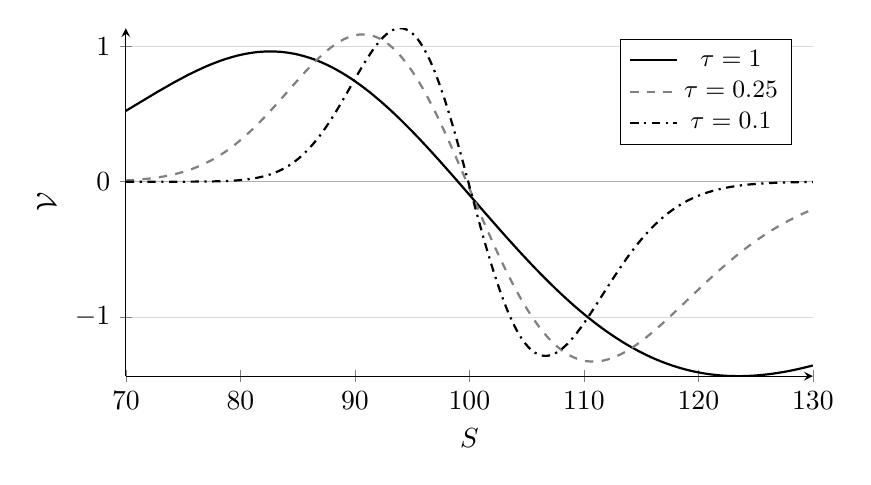
\begin{tikzpicture}
\begin{axis}[
    width=0.85\textwidth, height=6cm,
    xmin=70, xmax=130,
    xlabel={$S$}, ylabel={$\mathcal{V}$},
    ymajorgrids=true, grid style={gray!30},
    axis x line=bottom, axis y line=left,
    legend pos=north east, legend style={font=\small},
    samples=300,
    % Parameters: K = 100, r = 2%, q = 3%, sigma = 20%
    declare function={
      dtwo(\s,\t) = (ln(\s/100) - 0.03*\t)/(0.2*sqrt(\t));
      done(\s,\t) = dtwo(\s,\t) + 0.2*sqrt(\t);
      veg(\s,\t)  = -exp(-0.02*\t)*exp(-0.5*dtwo(\s,\t)*dtwo(\s,\t))*done(\s,\t)
                    /(sqrt(2*pi)*0.2);
    },
]
  \addplot[gray!60, thin, domain=70:130, forget plot] {0};
  \addplot[black, thick, domain=70:130] {veg(x,1)};
  \addlegendentry{$\tau = 1$}
  \addplot[gray, thick, dashed, domain=70:130] {veg(x,0.25)};
  \addlegendentry{$\tau = 0.25$}
  \addplot[black, thick, dash dot, domain=70:130] {veg(x,0.1)};
  \addlegendentry{$\tau = 0.1$}
\end{axis}
\end{tikzpicture}
\caption{Black--Scholes vega of a cash-or-nothing call ($Q=1$, $K=100$,
$r=2\%$, $q=3\%$, $\sigma=20\%$). Vega has the same sign pattern as gamma:
a rise in volatility helps the out-of-the-money digital and hurts the
in-the-money one.}
\label{fig:bs-digital-vega}
\end{figure}

% ---------------------------------------------------------------------
\subsection{American Digital Options}
\label{subsec:bs-american}

\subsubsection{Optimal Exercise and Equivalence with One-Touch Options}

An American cash-or-nothing call allows its holder to exercise at any stopping
time $\theta \in [t,T]$ and to receive $Q$ provided $S_\theta \geq K$. Let
$\tau_K = \inf\{u \geq t : S_u \geq K\}$ be the first hitting time of the
strike.

\begin{proposition}
\label{prop:american-one-touch}
If $r \geq 0$ and $S_t < K$, the American cash-or-nothing call is equivalent
to a one-touch option with barrier $B = K$ paying $Q$ at the hitting time:
\begin{equation}
  V^{\mathrm{Am}}_t = Q\,\mathbb{E}^{\mathbb{Q}}\!\left[e^{-r(\tau_K - t)}\,\mathbf{1}_{\{\tau_K \leq T\}} \mid \mathcal{F}_t\right].
  \label{eq:american-one-touch}
\end{equation}
\end{proposition}

\begin{proof}
Any exercise strategy pays only at a time $\theta$ such that
$S_\theta \geq K$, hence $\theta \geq \tau_K$. Since $r \geq 0$,
$e^{-r(\theta-t)} \leq e^{-r(\tau_K-t)}$, so no strategy is worth more than
the right-hand side of~\eqref{eq:american-one-touch}. The strategy
$\theta = \tau_K$ attains this bound.
\end{proof}

\begin{remark}
When $r < 0$, as was the case for euro rates between 2015 and 2022, delaying
the payment becomes valuable and the equivalence no longer holds. The same
argument then only gives the bounds
$\mathrm{OT}^{\mathrm{hit}} \leq V^{\mathrm{Am}} \leq \mathrm{OT}^{\mathrm{exp}}$,
where $\mathrm{OT}^{\mathrm{hit}}$ and $\mathrm{OT}^{\mathrm{exp}}$ are the
one-touch options paying at the hitting time and at maturity respectively.
\end{remark}

\subsubsection{One-Touch Paying at Hit}

Let $\eta = -1$ for an upper barrier ($S_t < B$) and $\eta = +1$ for a lower
barrier ($S_t > B$), and define
\begin{equation}
  \mu = \frac{\nu}{\sigma^2},
  \qquad
  \lambda = \sqrt{\mu^2 + \frac{2r}{\sigma^2}},
  \qquad
  z = \frac{\ln(B/S_t)}{\sigma\sqrt{\tau}} + \lambda\,\sigma\sqrt{\tau}.
\end{equation}
The price of a one-touch paying $Q$ at the hitting time
is~\cite{ReinerRubinstein1991,Haug2007}
\begin{equation}
  \mathrm{OT}^{\mathrm{hit}}
  = Q\left[\left(\frac{B}{S_t}\right)^{\mu+\lambda} N(\eta z)
  + \left(\frac{B}{S_t}\right)^{\mu-\lambda} N\!\left(\eta z - 2\eta\lambda\sigma\sqrt{\tau}\right)\right].
  \label{eq:one-touch-hit}
\end{equation}
By Proposition~\ref{prop:american-one-touch}, this is also the price of the
American digital call ($\eta=-1$, $B=K$) and, symmetrically, of the American
digital put ($\eta=+1$, $B=K$).

\subsubsection{One-Touch Paying at Maturity and No-Touch Options}

When the rebate is paid at maturity, the price is
$\mathrm{OT}^{\mathrm{exp}} = Q\,e^{-r\tau}\,\mathbb{Q}(\tau_B \leq T \mid \mathcal{F}_t)$.
Writing $x = \ln(S_t/B)$, the reflection principle for Brownian motion with
drift~\cite{Shreve2004} gives
\begin{equation}
  \mathbb{Q}(\tau_B \leq T \mid \mathcal{F}_t)
  = N\!\left(-\eta\,\frac{x + \nu\tau}{\sigma\sqrt{\tau}}\right)
  + \left(\frac{B}{S_t}\right)^{2\mu} N\!\left(-\eta\,\frac{x - \nu\tau}{\sigma\sqrt{\tau}}\right).
  \label{eq:touch-probability}
\end{equation}
A no-touch option, which pays $Q$ at maturity if the barrier is never reached,
follows by parity: $\mathrm{NT} = Q\,e^{-r\tau} - \mathrm{OT}^{\mathrm{exp}}$.

\subsubsection{Comparison with the European Digital}

When $\nu = 0$, \eqref{eq:touch-probability} reduces to
$\mathbb{Q}(\tau_B \leq T) = 2\,\mathbb{Q}(S_T \geq B)$ for an upper barrier:
a path that reaches the barrier has, by symmetry, one chance in two of ending
above it. Hence
\begin{equation}
  \mathrm{OT}^{\mathrm{exp}}(B) = 2\,D^{c}(K = B) \quad \text{when } \nu = 0.
  \label{eq:rule-of-thumb}
\end{equation}
For realistic parameters, $\nu$ is small and the market rule of thumb
``a one-touch is worth about twice the corresponding European digital''
remains a good approximation (Figure~\ref{fig:bs-one-touch}).

% --- Figure: one-touch vs European -------------------------------------
\begin{figure}[htbp]
\centering
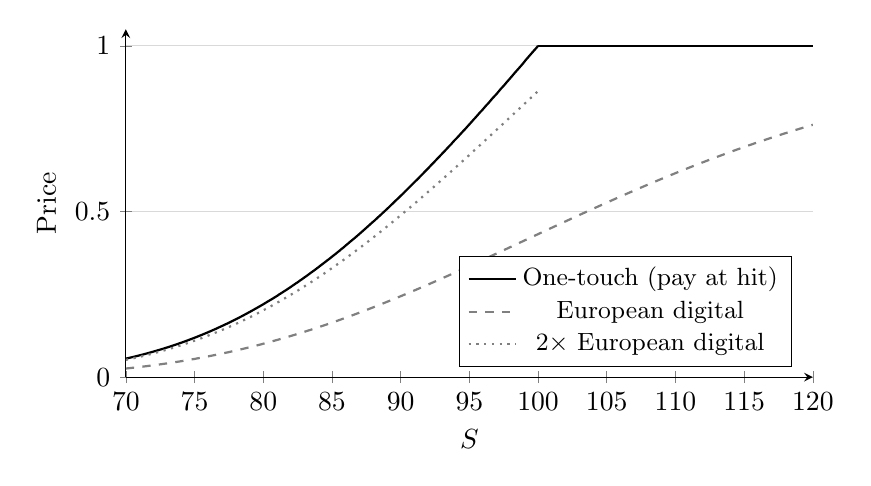
\begin{tikzpicture}
\begin{axis}[
    width=0.85\textwidth, height=6cm,
    xmin=70, xmax=120, ymin=0, ymax=1.05,
    xlabel={$S$}, ylabel={Price},
    ymajorgrids=true, grid style={gray!30},
    axis x line=bottom, axis y line=left,
    legend pos=south east, legend style={font=\small},
    samples=200,
    % Parameters: K = B = 100, tau = 1, r = 2%, q = 3%, sigma = 20%
    % mu = -0.75, lambda = 1.25
    declare function={
      Ncdf(\x) = 1/(1+exp(-0.07056*\x*\x*\x - 1.5976*\x));
      dtwo(\s) = (ln(\s/100) - 0.03)/0.2;
      zz(\s)   = ln(100/\s)/0.2 + 0.25;
      ot(\s)   = (100/\s)^0.5*Ncdf(-zz(\s)) + (100/\s)^(-2)*Ncdf(-zz(\s)+0.5);
    },
]
  \addplot[black, thick, domain=70:100] {ot(x)};
  \addlegendentry{One-touch (pay at hit)}
  \addplot[black, thick, domain=100:120, forget plot] {1};
  \addplot[gray, thick, dashed, domain=70:120] {exp(-0.02)*Ncdf(dtwo(x))};
  \addlegendentry{European digital}
  \addplot[gray, thick, dotted, domain=70:100] {2*exp(-0.02)*Ncdf(dtwo(x))};
  \addlegendentry{$2\times$ European digital}
\end{axis}
\end{tikzpicture}
\caption{Black--Scholes prices of a one-touch paying at hit and of a European
cash-or-nothing call ($Q=1$, $K=B=100$, $\tau=1$, $r=2\%$, $q=3\%$,
$\sigma=20\%$).}
\label{fig:bs-one-touch}
\end{figure}

% ---------------------------------------------------------------------
\subsection{Bermudan Digital Options}
\label{subsec:bs-bermudan}

A Bermudan cash-or-nothing call can only be exercised on a finite set of
observation dates $t < t_1 < \dots < t_m = T$. By the argument of
Proposition~\ref{prop:american-one-touch}, when $r \geq 0$ it is optimal to
exercise at the first observation date on which $S_{t_i} \geq K$. Writing
$s_i = t_i - t$, the price is
\begin{equation}
  V^{\mathrm{Berm}}_t = Q \sum_{i=1}^{m} e^{-r s_i}\,\bigl(F_{i-1} - F_i\bigr),
  \qquad F_0 = 1,
  \label{eq:bermudan-price}
\end{equation}
where
$F_i = \mathbb{Q}\left(S_{t_1} < K, \dots, S_{t_i} < K \mid \mathcal{F}_t\right)$
is the probability that the option has not been exercised after $i$
observations. Under~\eqref{eq:bs-sde}, $F_i$ is an $i$-dimensional normal
distribution function:
\begin{equation}
  F_i = \Phi_i\left(a_1, \dots, a_i;\, R_i\right),
  \qquad
  a_j = \frac{\ln(K/S_t) - \nu s_j}{\sigma\sqrt{s_j}},
  \qquad
  (R_i)_{jl} = \sqrt{\frac{s_{\min(j,l)}}{s_{\max(j,l)}}}.
  \label{eq:bermudan-cdf}
\end{equation}
For $m=1$, \eqref{eq:bermudan-price} reduces to the European
price~\eqref{eq:cash-call}. For a moderate number of dates, as for the annual
observations of an autocall, the multivariate normal distribution can be
evaluated numerically. For frequent monitoring, Monte Carlo simulation or the
continuity correction of Broadie, Glasserman and Kou~\cite{BroadieGlassermanKou1997}
is preferred: with equally spaced dates $\Delta t$ apart, the Bermudan digital
is approximated by the one-touch~\eqref{eq:one-touch-hit} with the barrier
shifted away from the spot,
\begin{equation}
  B^{\star} = K\,e^{-\eta\,\beta\,\sigma\sqrt{\Delta t}},
  \qquad
  \beta = -\frac{\zeta(1/2)}{\sqrt{2\pi}} \approx 0.5826,
  \label{eq:bgk}
\end{equation}
where $\zeta$ is the Riemann zeta function.

Since a Bermudan digital whose last date is $T$ can be exercised whenever the
European digital pays, and at least as early, the three exercise styles are
ordered for $r \geq 0$:
\begin{equation}
  D^{c} \;\leq\; V^{\mathrm{Berm}} \;\leq\; V^{\mathrm{Am}}.
  \label{eq:ordering}
\end{equation}
The observation frequency therefore interpolates continuously between the
European and the American digital.

% ---------------------------------------------------------------------
\subsection{Limitations of the Black--Scholes Framework}
\label{subsec:bs-limits}

The formulas above are exact under the assumptions of the model, but these
assumptions are particularly restrictive for digital options on an equity
index.

\begin{enumerate}
  \item \textbf{No smile.} The model uses a single volatility, whereas the
        market quotes a skewed implied volatility surface. As shown
        by~\eqref{eq:smile-correction}, the price of a European digital
        depends on the slope of the smile at the strike, which no choice of a
        single $\sigma$ can capture consistently across strikes.
  \item \textbf{No volatility dynamics.} American and Bermudan digitals depend
        on the whole path of the underlying. Their prices are determined not
        only by today's surface but by its future evolution (forward skew,
        volatility of volatility, spot--volatility correlation), which the
        Black--Scholes model fixes by assumption.
  \item \textbf{Hedging instability.} The unbounded delta and gamma near the
        strike at maturity make the theoretical delta hedge impossible to
        implement. In practice, digitals are hedged and priced conservatively
        with call spreads, as in~\eqref{eq:call-spread-limit}, at a cost that
        depends on the smile.
\end{enumerate}

These limitations motivate the stochastic volatility model presented in
Section~\ref{sec:heston}, in which the spot--volatility correlation generates
a skew and the volatility of volatility governs the path-dependent effects.

% ==================================================================
\section{Market Data and Model}
\label{sec:data}
% ==================================================================

\subsection{Data}

As usual, the data used in this paper are available on my
website\footnote{\url{https://portfolio-eliasbenguedda.fr}}. We use CAC~40
option quotes of 12 February 2025 to build an implied volatility surface.

\subsection{Model}

We use the Heston model, previously calibrated to this
surface\footnote{\url{https://portfolio-eliasbenguedda.fr/projects/Heston.html}}.

% ==================================================================
\section{Pricing under the Heston Model}
\label{sec:heston}
% ==================================================================

As seen in the previous section, the Black--Scholes model is

\subsection{Cash-or-Nothing Options}

\subsubsection{European Style}

\subsubsection{American Style}

\subsubsection{Bermudan Style}

% ==================================================================
\section{Greeks}
\label{sec:greeks}
% ==================================================================

% ==================================================================
\section{Hedging of a Digital}
\label{sec:hedging}
% ==================================================================

As shown in Section~\ref{subsec:call-spread}, a digital option can be hedged
and priced with a call spread. The remaining question is: which call spread?

% ==================================================================
\clearpage
\begin{thebibliography}{99}

\bibitem{BlackScholes1973}
F.~Black and M.~Scholes,
The Pricing of Options and Corporate Liabilities,
\emph{Journal of Political Economy}, 81(3):637--654, 1973.

\bibitem{BroadieGlassermanKou1997}
M.~Broadie, P.~Glasserman and S.~Kou,
A Continuity Correction for Discrete Barrier Options,
\emph{Mathematical Finance}, 7(4):325--349, 1997.

\bibitem{Bouzoubaa2010}
M.~Bouzoubaa and A.~Osseiran,
\emph{Exotic Options and Hybrids: A Guide to Structuring, Pricing and Trading},
Wiley, 2010.
\url{https://www.academia.edu/40236904/Exotic_Options_And_Hybrids_1_}

\bibitem{Haug2007}
E.~G.~Haug,
\emph{The Complete Guide to Option Pricing Formulas}, 2nd edition,
McGraw-Hill, 2007.

\bibitem{Merton1973}
R.~C.~Merton,
Theory of Rational Option Pricing,
\emph{Bell Journal of Economics and Management Science}, 4(1):141--183, 1973.

\bibitem{ReinerRubinstein1991}
E.~Reiner and M.~Rubinstein,
Unscrambling the Binary Code,
\emph{Risk}, 4(9):75--83, 1991.

\bibitem{Shreve2004}
S.~E.~Shreve,
\emph{Stochastic Calculus for Finance II: Continuous-Time Models},
Springer, 2004.

\end{thebibliography}

\end{document}
